% ============================================================================
% AI-Assisted Master Prompt Generation — Thesis Defense
% Built on the metropolis beamer theme (github.com/matze/mtheme), not a
% hand-rolled one: metropolis already provides correct, well-tested
% mechanics for the title page, frametitle sizing, and per-frame vertical
% centering (its inner theme explicitly patches around a beamer core glue
% bug -- \beamer@initfirstlineunskip -- that broke a from-scratch [c]
% implementation earlier in this deck's history). Colors, box styles, the
% footer (logo + rule), and all slide content are unchanged from before;
% only the underlying scaffolding is now the standard theme instead of
% custom \setbeamertemplate overrides for things metropolis already does.
%
% Compile: pdflatex defense.tex  (run twice for the outline/TOC to settle)
% ============================================================================
\documentclass[aspectratio=169,11pt,c]{beamer}
% 11pt (was 10pt): a uniform bump so everything -- body text, quotes,
% tables, footer -- scales up together for projection/visibility, rather
% than only enlarging a few hand-picked elements.
% 'c': metropolis's inner theme redefines the underlying beamerframe 'c'
% key (see beamerinnerthememetropolis.sty) to also neutralize
% \beamer@initfirstlineunskip -- the beamer-core glue behavior that made
% a from-scratch [c] implementation a no-op earlier in this deck's
% history. Verifying this actually centers before trusting it (below).
\usetheme[progressbar=none, sectionpage=progressbar]{metropolis}
% progressbar=none: this deck's own orange footer rule is the separator
%   on CONTENT slides, not metropolis's proportional progress bar --
%   avoids two competing orange lines on the same slide.
% sectionpage=progressbar: metropolis's built-in section-divider slide,
%   auto-inserted on every \section{} -- gives a clear "which part are we
%   in now" marker at each transition, with a thin orange progress bar
%   (reuses the \setbeamercolor{progress bar} set below) showing how far
%   through the talk that transition falls. Template-native, not custom.

\usepackage[T1]{fontenc}
\usepackage{helvet}
\renewcommand{\familydefault}{\sfdefault}
\usepackage{amssymb}
\usepackage{graphicx}
\graphicspath{{assets/}}
\usepackage{xcolor}
\usepackage{tikz}
\usetikzlibrary{arrows.meta,positioning,fit,backgrounds}
\usepackage{booktabs}
\usepackage{array}
\usepackage{tcolorbox}
\usepackage{ragged2e}
% Block ugly mid-word breaks (e.g. "speci-fication", "require-ment") on this
% deck's most frequent long words -- narrow columns (figpanel/quotebox/table
% cells) otherwise pick valid but visually awkward hyphenation points. A
% word listed with NO internal hyphens is never broken (previous version of
% this line listed *allowed* break points instead, which is backwards and
% still let "require-ment" through in narrow table columns).
\hyphenation{specification specifications consolidation requirement requirements traceability implementation reconstruction revises History before exclusion Lifecycle instructions semantic decomposition conflict conflicts values introduced}

% ---------------------------------------------------------------- palette --
% Unchanged from the previous version. Blue brightened from an original
% 1F4E79 -- at thin strokes (checkmarks, table digits) that navy read
% almost as black, undercutting the blue/orange/black balance. 2568A2
% stays professional but is unmistakably blue next to inkgray.
\definecolor{primaryblue}{HTML}{2568A2}
\definecolor{deepblue}{HTML}{123049}
\definecolor{accentorange}{HTML}{E08E2B}
\definecolor{tintblue}{HTML}{EAF1F8}
\definecolor{tintorange}{HTML}{FBE9D3}
\definecolor{inkgray}{HTML}{262A33}
\definecolor{midgray}{HTML}{707A8A}
\definecolor{linegray}{HTML}{D8DEE6}

% ---------------------------------------------------- map onto metropolis --
% metropolis exposes these as its customization hooks (read directly from
% beamercolorthememetropolis.sty): normal text drives most derived colors,
% frametitle/progress bar/title separator are the other hooks that matter
% here. Setting them after \usetheme is what overrides the theme's own
% defaults -- order matters in beamer color resolution.
\setbeamersize{text margin left=12mm,text margin right=12mm}
\setbeamercolor{normal text}{fg=inkgray,bg=white}
\setbeamercolor{structure}{fg=primaryblue}
\setbeamercolor{alerted text}{fg=accentorange}
\setbeamercolor{example text}{fg=primaryblue}
\setbeamercolor{frametitle}{fg=inkgray,bg=tintblue}
\setbeamercolor{title separator}{fg=accentorange}
\setbeamercolor{progress bar}{fg=accentorange,bg=linegray}
\setbeamercolor{titlelike}{fg=primaryblue}
% Title/subtitle uppercase and matched in size (explicit prior requirement)
% -- metropolis's stock templates render them mixed-case with the subtitle
% noticeably smaller, so both are overridden here; everything else about
% the title page (vfill centering, separator rule, author/date/institute
% stack) stays exactly as metropolis provides it.
\setbeamerfont{title}{size=\Large,series=\bfseries}
\setbeamerfont{subtitle}{size=\Large,series=\bfseries}
\setbeamertemplate{title}{%
  \centering
  {\scriptsize\color{midgray}\MakeUppercase{Bachelor's Thesis Defense}}\\[8pt]
  \linespread{1.0}\MakeUppercase{\inserttitle}\par\vspace*{0.5em}
}
% "Bachelor's Thesis Defense" moved here from \institute (it used to read
% as just another fact in the university/supervisor list, same size/color
% as everything else). As a small eyebrow directly above the title -- a
% standard academic title-slide convention -- it reads as a label for the
% whole page instead of blending into the institute block.
\setbeamertemplate{subtitle}{\centering\MakeUppercase{\insertsubtitle}\par\vspace*{0.5em}}
% \centering doesn't carry across separate \usebeamertemplate* calls (each
% one turned out to reset alignment on its own), so author/date/institute
% need the same treatment -- otherwise only the title/subtitle end up
% centered while the rest of the title page stays left-aligned. Bodies are
% unchanged from metropolis's stock templates; only \centering is added.
\setbeamerfont{author}{size=\large}
\setbeamerfont{date}{size=\normalsize}
\setbeamertemplate{author}{\centering\vspace*{2em}\insertauthor\par\vspace*{0.25em}}
\setbeamertemplate{date}{\centering\insertdate\par}
% author/date bumped to match institute's \normalsize below -- they were
% left at metropolis's smaller defaults, so the block read as inconsistent
% once institute grew. Author a notch larger (\large) since the name is
% the most prominent personal identifier on the page.
\setbeamerfont{institute}{size=\normalsize}
\setbeamertemplate{institute}{\centering\vspace*{3mm}\insertinstitute\par}
% \insertinstitute holds a left-aligned tabular for the two supervisor
% lines (so "Supervisor 1"/"Supervisor 2" start at the same x-position
% instead of each drifting to a different spot under independent
% centering), with the whole tabular then centered on the page as one
% block -- see \institute{} below.
\setbeamercolor{block title}{fg=primaryblue,bg=tintblue}
\setbeamercolor{block body}{fg=inkgray,bg=tintblue}
\setbeamerfont{frametitle}{series=\bfseries,size=\Large}
\setbeamertemplate{itemize item}{\textcolor{midgray}{--}}
\setbeamertemplate{itemize subitem}{\textcolor{midgray}{\textperiodcentered}}
\setbeamertemplate{caption}[numbered]
% Deliberately not touching \setbeamertemplate{frametitle}: metropolis's
% own (beamerouterthememetropolis.sty) already renders only the title --
% no subtitle line -- sizes itself via an invisible strut rather than a
% fixed height (so two-line backup-slide titles can't get clipped the way
% the earlier hand-rolled version did), and paints its bg edge-to-edge
% while keeping text indented to the margin. Recoloring it above is enough.

% ------------------------------------------------------------- footline ---
% metropolis has no built-in logo slot in the footline, so this part is
% still a custom override.
% The logo asset (assets/VGU-Logo.png) is a single flat lockup: the
% compact "VGU" mark plus "Vietnamese-German University" laid out as ONE
% long line spanning nearly the full 4726x1345 canvas (verified with PIL:
% the file has almost no wasted transparent margin, so cropping it doesn't
% help). Sizing it by height=0.4cm scaled that whole wide canvas down to a
% ~1.4cm width, crushing the caption line to a couple of points tall and
% making it illegible. Sizing by WIDTH instead keeps the caption readable;
% ht=3.6ex/dp=1.6ex on the box already has enough room (~0.79cm) for the
% resulting ~0.57cm-tall logo, so the compact footer band doesn't need to
% grow to fit it. leftskip=3mm keeps it snug in the bottom-left corner
% without touching the page edge.
\setbeamertemplate{footline}{%
  {\color{accentorange}\rule{\paperwidth}{1pt}}\\[16pt]
  \leavevmode
  \hbox{\begin{beamercolorbox}[wd=\paperwidth,ht=3.6ex,dp=1.6ex,leftskip=3mm,rightskip=10mm]{footline}
    \raisebox{-0.15cm}{
\includegraphics[width=1.7cm]{VGU-Logo.png}}
    \hfill
    {\scriptsize\bfseries\color{inkgray}\insertsection}
    \hfill
    {\scriptsize\bfseries\color{inkgray}\insertframenumber}
  \end{beamercolorbox}}
  \vspace{4pt}
}

% Bold centered orange one-liner, for a single punchy takeaway per slide.
\newcommand{\takeaway}[1]{\begin{center}{\bfseries\color{accentorange}\large #1}\end{center}}

% Title page: using metropolis's own template (beamerinnerthememetropolis.
% sty) via \maketitle instead of a hand-rolled one -- it already does
% title / separator rule / author / date / institute inside a \vfill-
% centered minipage, which is the same idiom the earlier custom version
% used, just theme-provided instead of reimplemented. The "Bachelor's
% Thesis Defense" label now lives as the first line of \institute below,
% since metropolis's stock template has no separate eyebrow slot.

% ----------------------------------------------------------- box styles --
\newtcolorbox{quotebox}{%
  colback=white, colframe=accentorange, boxrule=0pt, leftrule=2.4pt,
  arc=0pt, outer arc=0pt, boxsep=1pt, left=8pt, right=8pt, top=3pt, bottom=3pt,
  fontupper=\small\color{inkgray}
}
\newtcolorbox{calloutbox}{%
  colback=tintblue, colframe=linegray, boxrule=0.6pt, arc=2pt,
  left=8pt, right=8pt, top=3pt, bottom=3pt, fontupper=\small\color{inkgray}
}
% quotebox/calloutbox kept at \small rather than bumped to \normalsize:
% at the new 11pt base, \small is already larger than it was at 10pt, and
% \normalsize specifically overflowed the denser frames (bullets + diagram
% + callout together) past the footer -- verified by rendering, not
% assumed.
% Dashed frame drawn behind a diagram's nodes (via fit+backgrounds), fitted
% and padded automatically -- matches the reference slide's dotted-border
% boxes around its Workflow/Agent figures. Usage inside a tikzpicture,
% after all the flow nodes are placed: \diagramframe{(n1)(n2)(n3)...}
\newcommand{\diagramframe}[1]{%
  \begin{pgfonlayer}{background}
    \node[draw=linegray, dashed, rounded corners=4pt, inner sep=10pt, fill=white, fit=#1] {};
  \end{pgfonlayer}%
}
\newtcolorbox{flagpanel}{%
  colback=tintorange, colframe=accentorange, boxrule=0.6pt, arc=2pt,
  left=6pt, right=6pt, top=2pt, bottom=2pt, fontupper=\footnotesize\color{inkgray}
}
\newtcolorbox{goodpanel}{%
  colback=tintblue, colframe=primaryblue, boxrule=0.6pt, arc=2pt,
  left=6pt, right=6pt, top=5pt, bottom=5pt, fontupper=\footnotesize\color{inkgray}
}
% Bordered white card (thin gray rule, no fill) for framing a small
% conceptual figure -- the "research-paper figure panel" look.
\newtcolorbox{figpanel}{%
  colback=white, colframe=linegray, boxrule=0.6pt, arc=3pt,
  left=5pt, right=5pt, top=2pt, bottom=2pt, boxsep=0pt
}
\newcommand{\quotewho}[1]{{\footnotesize\bfseries\color{accentorange}\MakeUppercase{#1}}\\[2pt]}
\newcommand{\calllbl}[1]{{\footnotesize\bfseries\color{primaryblue}\MakeUppercase{#1}}\\[2pt]}
\newcommand{\panelwho}[1]{{\bfseries\color{inkgray}#1}\\[2pt]}

\tikzset{
  flownode/.style={draw=linegray,rounded corners=2pt,fill=tintblue,inner sep=5pt,font=\scriptsize,text=inkgray},
  flowarrow/.style={-{Latex[length=2mm]},draw=accentorange,thick},
  msgnode/.style={draw=linegray,rounded corners=2pt,fill=white,inner sep=4pt,font=\tiny,text=inkgray},
}
% Small flat icons for the human/AI conceptual-figure diagrams: a plain
% person glyph (circle head + trapezoid body, no asset needed) paired with
% the actual model icon that produced the shown output -- not a generic
% robot -- so the figure reads as a real result, not a mockup.
\newcommand{\humanicon}{%
  
\begin{tikzpicture}[baseline=-0.5ex]
    \fill[midgray] (0,0.20) circle (0.085);
    \fill[midgray] (-0.13,-0.20) -- (0.13,-0.20) -- (0.17,0.06) -- (-0.17,0.06) -- cycle;
  \end{tikzpicture}%
}
\newcommand{\aiicon}[1]{\includegraphics[width=0.5cm]{#1}}

% ----------------------------------------------------------------- meta --
\title{AI-Assisted Master Prompt Generation}
\subtitle{Challenges and Proposed Solutions}
\author{Nguyen Thanh Tu \textbar\ Student ID 10422080}
\institute{%
  \begin{tabular}{l}
    Supervisor 1: Assoc.\ Prof.\ Garcia Clavel Manuel \\
    Supervisor 2: Dr.\ Nguyen Tuan Cuong
  \end{tabular}\\[8pt]
  Computer Science, Vietnamese--German University
}
\date{17 August 2026}

\begin{document}

\maketitle

\begin{frame}{Outline}
  \framesubtitle{What we'll cover}
  \tableofcontents
\end{frame}

% ============================================================ SECTION 1 ==
\section{Motivation \& Problem}

\begin{frame}{What Is a Master Prompt?}
  \framesubtitle{Problem}
  \begin{center}
  
\begin{tikzpicture}[node distance=4mm]
    \node[flownode,text width=1.5cm,align=center] (p1) {Prompt 1};
    \node[flownode,right=of p1,text width=1.5cm,align=center] (p2) {Prompt 2};
    \node[flownode,right=of p2,text width=1.5cm,align=center] (p3) {Prompt 3};
    \node[right=of p3,font=\bfseries\color{midgray}] (dots) {\dots};
    \node[flownode,right=of dots,text width=1.5cm,align=center] (pn) {Prompt N};
    \node[flownode,right=of pn,fill=tintorange,draw=accentorange,text width=2.4cm,align=center] (mp) {\textbf{MASTER PROMPT}};
    \draw[flowarrow] (p1)--(p2); \draw[flowarrow] (p2)--(p3); \draw[flowarrow] (p3)--(dots); \draw[flowarrow] (dots)--(pn); \draw[flowarrow] (pn)--(mp);
  \end{tikzpicture}
  \end{center}
  \vspace{1pt}
  \footnotesize
  \begin{itemize}
    \item Requirements evolve across prompts through additions, modifications, replacements, and removals.
    \item A master prompt captures the user's currently valid intent --- not the entire conversation history.
    \item It consolidates the evolving requirements into one self-contained specification that can be reused across sessions, agents, or developers.
    \item It keeps only final active requirements and remove all unsupported details.
  \end{itemize}
  \begin{calloutbox}
    \footnotesize\calllbl{Definition}A \textbf{master prompt} is a single, self-contained specification of the user's currently valid intent.
  \end{calloutbox}
\end{frame}

\begin{frame}{A Master Prompt Is Not Exactly a Conversation Summary}
  \framesubtitle{Problem}
  \begin{flagpanel}
    \footnotesize ``Build a \textbf{single-page} portal homepage \textbf{as a static site using only plain HTML, CSS, and vanilla JavaScript (three files: index.html, style.css, app.js)} --- \textbf{no frameworks or build step}. Layout \& navigation: use a horizontal top navigation bar \underline{\textbf{(no sidebar)}} \textbf{with a brand/logo on the left and the nav buttons on the right.} Include exactly four navigation buttons: Dashboard, Policies, History, Contact. \textbf{Clicking a button switches between four corresponding in-page views without reloading; the active button is highlighted.}''
  \end{flagpanel}
  \vspace{2pt}
  {\scriptsize
  \textbf{Error 1 --- Unsupported details (extrinsic hallucination)} (\textbf{bold}): details introduced during consolidation that are not supported by the user's prompt history.\\[2pt]
  \textbf{Error 2 --- Inactive constraint} (\underline{\textbf{underlined}}): the sidebar was removed earlier, but stating ``no sidebar'' not an active requirement in the ground-truth Master Prompt..
  }
  \vspace{2pt}
  \begin{center}\scriptsize\raisebox{-0.06cm}{\aiicon{claude-icon.png}}\ \textbf{Claude \textperiodcentered\ simple project \textperiodcentered\ basic consolidation --- AlignScore 0.086, 92\% untraceable}\end{center}
\end{frame}

\begin{frame}{From Prompt History to a Master Prompt}
  \framesubtitle{Problem}
  \begin{columns}[T]
    \begin{column}{0.44\textwidth}
      \begin{figpanel}
        \begin{center}\humanicon\end{center}
        \begin{itemize}\scriptsize
          \item ``Create a portal homepage.''
          \item ``Add 3 navigation buttons: Home, Orders, Contact.''
          \item ``Add sidebar navigation.''
          \item ``Undo sidebar.'' \textcolor{accentorange}{\textbf{(undo)}}
          \item ``Use top navigation instead.'' \textcolor{accentorange}{\textbf{(replace)}}
          \item ``Change navigation buttons: Dashboard, Policies, History, Contact.'' \textcolor{accentorange}{\textbf{(replace)}}
        \end{itemize}
      \end{figpanel}
    \end{column}
    \begin{column}{0.08\textwidth}
      \begin{center}
        \vspace{1.2cm}
        \aiicon{claude-icon.png}\\[2pt]
        {\tiny\color{midgray}consolidate}\\[1pt]
        {\large$\Longrightarrow$}
      \end{center}
    \end{column}
    \begin{column}{0.44\textwidth}
      \begin{figpanel}
        \begin{center}\footnotesize\bfseries\color{inkgray}Expected Master Prompt\end{center}
        \vspace{4pt}
        \begin{quotebox}
          \centering\scriptsize ``Create a portal homepage. Add top navigation. The navigation must contain four buttons: Dashboard, Policies, History, and Contact.''
        \end{quotebox}
      \end{figpanel}
    \end{column}
  \end{columns}
  \vspace{1pt}
  \takeaway{A master prompt is not a summary of everything the user said --- it is a specification of what is still valid at the end of the history.}
\end{frame}

\begin{frame}{Properties of a Reliable Master Prompt}
  \framesubtitle{Problem}
  \begin{itemize}
    \item \textbf{Faithful} --- every requirement is supported by the user's prompt history; unsupported additions or extrinsic hallucinations are excluded.
    \item \textbf{Current} --- later modifications, removals, and replacements are reflected in the final specification.
    \item \textbf{Conflict-aware} --- if a later instruction conflicts with a settled requirement without clearly requesting a revision, surface the conflict instead of silently changing the requirement.
  \end{itemize}
\end{frame}

% ============================================================ SECTION 2 ==
\section{Research Questions \& Contributions}

\begin{frame}{Research Questions}
  \framesubtitle{Research Questions}
  \begin{itemize}
    \item \textbf{RQ1} --- To what extent do AI-generated master prompts contain non-traceable content, including agent-added and outdated requirements, and how does consolidation instruction strictness affect this problem?
    \item \textbf{RQ2} --- Does spec-guided consolidation produce a more traceable master prompt than single-pass consolidation of the raw prompt history?
    \item \textbf{RQ3} --- When a later instruction semantically conflicts with a settled requirement, how can a spec-guided approach surface the conflict, trace both sides, and avoid resolving it without user input?
  \end{itemize}
\end{frame}

\begin{frame}{Contributions}
  \framesubtitle{Contributions}
  \begin{itemize}
    \item \textbf{Requirement-level traceability evaluation} --- a requirement-level method using atomic decomposition and entailment-based AlignScore to evaluate whether candidate master-prompt requirements are supported by the ground truth.
    \item \textbf{Spec-guided consolidation} --- a maintained specification is updated throughout the prompt history rather than reconstructed only at the end.
    \item \textbf{Conflict-aware project handoff} --- later instructions are checked against the settled specification; unclear conflicts are preserved for user resolution rather than silently resolved.
  \end{itemize}
\end{frame}

% ============================================================ SECTION 4 ==
\section{Related Work}

\begin{frame}{Related Work}
  \framesubtitle{Related Work}
  \small
  \begin{itemize}
    \item \textbf{Mondal et al.\ (2024) --- \textit{Enhancing User Interaction in ChatGPT}} --- combines sequences of prompts into one prompt; the main goal is interaction efficiency. Does not evaluate requirement-level traceability or later undo/replacement behavior.
    \item \textbf{AlignScore / FActScore / Claimify} --- provide ideas for semantic support and atomic evaluation. Do not construct or maintain a master prompt.
    \item \textbf{Spec-driven development} --- treats a specification as a maintained artifact. Does not directly evaluate unsupported or outdated requirements in an AI-generated master prompt.
  \end{itemize}
\end{frame}

\begin{frame}{Closest Prior Work: Semantic Commit}
  \framesubtitle{Related Work}
  \begin{itemize}
    \item \textbf{Semantic Commit} checks new information for semantic conflicts before updating an intent specification and can suggest resolutions for user review.
    \item \textbf{My thesis:} studies the construction of a Master Prompt that remains traceable to the original  prompt history.
    \item For unclear conflicts, the settled requirement is preserved, trace back to requirement that cause conflicts, and the user is asked to decide rather than automatically choosing or merging them.
  \end{itemize}
\end{frame}

% ============================================================ SECTION 5 ==
\section{Methodology}

\begin{frame}{Experimental Design: Two Stages of the Master-Prompt Lifecycle}
  \framesubtitle{Methodology}
  \begin{columns}[T]
    \begin{column}{0.49\textwidth}
      {\small\bfseries\color{primaryblue}Master-Prompt Construction}
      \vspace{2pt}
      {\scriptsize\itshape\color{inkgray}``Can a traceable master prompt be constructed from an evolving prompt history?''\par}
      \vspace{5pt}
      \begin{itemize}\scriptsize
        \item \textbf{Input:} 2 project histories
        \item \textbf{Process:} 4 consolidation strategies $\times$ 3 AI coding agents
        \item \textbf{Output:} candidate master prompts
        \item \textbf{Evaluation:} requirement-level traceability (AlignScore + untraceable rate)
      \end{itemize}
    \end{column}
    \begin{column}{0.49\textwidth}
      {\small\bfseries\color{primaryblue}Semantic Conflict Handling}
      \vspace{2pt}
      {\scriptsize\itshape\color{inkgray}``Can later semantic conflicts be surfaced without silently changing a settled master prompt?''\par}
      \vspace{5pt}
      \begin{itemize}\scriptsize
        \item \textbf{Input:} hand-written ground-truth master prompt as settled specification + later prompts
        \item \textbf{Process:} 3 conflict-handling conditions $\times$ the same 3 AI coding agents
        \item \textbf{Output:} updated specification / conflict-handling behavior
        \item \textbf{Evaluation:} qualitative review (RQ3)
      \end{itemize}
    \end{column}
  \end{columns}
  \vspace{6pt}
  \takeaway{Experiment 1 uses ground truth as a scoring reference. Experiment 2 reuses it as the settled starting specification.}
\end{frame}

\begin{frame}{Two Controlled Project Histories and Ground Truth}
  \framesubtitle{Methodology}
  \begin{center}\scriptsize
  \begin{tabular}{lcp{7.4cm}}
    \toprule
    \textbf{Project} & \textbf{Prompts} & \textbf{Description} \\
    \midrule
    Simple & 12 & Portal with navigation, conditional styling, and contact form \\
    \addlinespace[3pt]
    Hard & 45 & ERP-style application with customers, orders, invoices, roles, and permissions; more revisions and removals \\
    \bottomrule
  \end{tabular}
  \end{center}
  \vspace{2pt}
  \begin{calloutbox}
    \scriptsize\calllbl{Ground truth}Manually constructed from the ordered history: retains only requirements still valid at the end; later modifications replace earlier values; removals/undo remove the affected requirement; unsupported details are excluded.
  \end{calloutbox}
  \vspace{2pt}
  {\small\color{midgray}\centering For Experiment 1, the ground-truth master prompt is also manually decomposed into atomic requirements.\par}
\end{frame}

% ============================================================ SECTION 6 ==
\section{Experiment 1: Traceability Evaluation}

\begin{frame}{Experiment 1 Pipeline}
  \framesubtitle{Experiment 1 --- Traceability Evaluation}
  \begin{center}
  
\begin{tikzpicture}[node distance=2.5mm]
    \node[flownode,inner sep=3pt,font=\tiny,text width=1.85cm,align=center] (p1) {1. prompt history};
    \node[flownode,inner sep=3pt,font=\tiny,right=of p1,text width=1.85cm,align=center] (p2) {2. consolidation strategy};
    \node[flownode,inner sep=3pt,font=\tiny,right=of p2,text width=1.85cm,align=center] (p3) {3. candidate master prompt};
    \node[flownode,inner sep=3pt,font=\tiny,right=of p3,text width=1.85cm,align=center] (p4) {4. atomic requirement decomposition};
    \node[flownode,inner sep=3pt,font=\tiny,right=of p4,text width=1.85cm,align=center] (p5) {5. AlignScore vs.\ ground truth};
    \node[flownode,inner sep=3pt,font=\tiny,right=of p5,fill=tintorange,draw=accentorange,text width=1.85cm,align=center] (p6) {6. results \& interpretation};
    \draw[flowarrow] (p1)--(p2); \draw[flowarrow] (p2)--(p3); \draw[flowarrow] (p3)--(p4);
    \draw[flowarrow] (p4)--(p5); \draw[flowarrow] (p5)--(p6);
  \end{tikzpicture}
  \end{center}
  \vspace{10pt}
  \takeaway{2 histories $\times$ 3 agents $\times$ 4 strategies = 24 candidates.}
\end{frame}

\begin{frame}{Four Consolidation Strategies}
  \framesubtitle{Experiment 1 --- Traceability Evaluation}
  \begin{columns}[T]
    \begin{column}{0.5\textwidth}
      {\small\bfseries\color{inkgray}Group A --- Single-pass}
      {\scriptsize\color{midgray}\quad P1 $\to$ \dots $\to$ P$N$ $\to$ consolidate once\par}
      \begin{itemize}\scriptsize
        \item \textbf{Basic} --- consolidate the conversation once at the end.
        \item \textbf{Loose} --- additionally account for modifications, removals, and missing/additional features.
        \item \textbf{Strict} --- additionally require every requirement to be traceable to the prompt history.
      \end{itemize}
      \vspace{2pt}
      {\small\bfseries\color{inkgray}Group B --- Per-turn}
      {\scriptsize\color{midgray}\quad P1, P2, \dots, P$N$ $\to$ update spec after each\par}
      \begin{itemize}\scriptsize
        \item \textbf{Spec-guided} --- before the prompt history begins, give the agent a governance instruction to maintain \texttt{prompts.md} and \texttt{spec.md}; after each new prompt, update the current specification.
      \end{itemize}
    \end{column}
    \begin{column}{0.46\textwidth}
      \begin{center}
      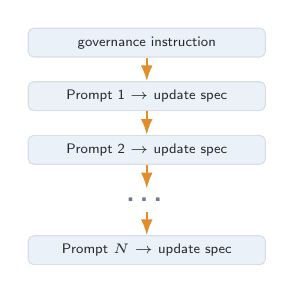
\begin{tikzpicture}[node distance=3mm]
        \node[flownode,inner sep=3pt,font=\tiny,text width=2.8cm,align=center] (g0) {governance instruction};
        \node[flownode,inner sep=3pt,font=\tiny,below=of g0,text width=2.8cm,align=center] (g1) {Prompt 1 $\to$ update spec};
        \node[flownode,inner sep=3pt,font=\tiny,below=of g1,text width=2.8cm,align=center] (g2) {Prompt 2 $\to$ update spec};
        \node[below=of g2,font=\bfseries\color{midgray}] (gdots) {\dots};
        \node[flownode,inner sep=3pt,font=\tiny,below=of gdots,text width=2.8cm,align=center] (gn) {Prompt $N$ $\to$ update spec};
        \draw[flowarrow] (g0)--(g1); \draw[flowarrow] (g1)--(g2); \draw[flowarrow] (g2)--(gdots); \draw[flowarrow] (gdots)--(gn);
      \end{tikzpicture}
      \end{center}
    \end{column}
  \end{columns}
\end{frame}

\begin{frame}{Challenge: Defining the Evaluation Unit}
  \framesubtitle{Experiment 1 --- Traceability Evaluation}
  \begin{columns}[T]
    \begin{column}{0.48\textwidth}
      \begin{center}{\small\bfseries\color{inkgray}Ground truth}\end{center}
      \begin{center}
      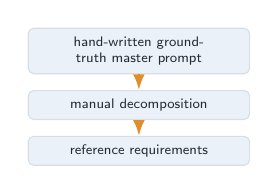
\begin{tikzpicture}[node distance=2mm]
        \node[flownode,inner sep=3pt,font=\tiny,text width=2.6cm,align=center] (g1) {hand-written ground-truth master prompt};
        \node[flownode,inner sep=3pt,font=\tiny,below=of g1,text width=2.6cm,align=center] (g2) {manual decomposition};
        \node[flownode,inner sep=3pt,font=\tiny,below=of g2,text width=2.6cm,align=center] (g3) {reference requirements};
        \draw[flowarrow] (g1)--(g2); \draw[flowarrow] (g2)--(g3);
      \end{tikzpicture}
      \end{center}
    \end{column}
    \begin{column}{0.48\textwidth}
      \begin{center}{\small\bfseries\color{inkgray}Candidate}\end{center}
      \begin{center}
      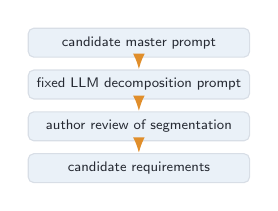
\begin{tikzpicture}[node distance=1.5mm]
        \node[flownode,inner sep=3pt,font=\tiny,text width=2.6cm,align=center] (d1) {candidate master prompt};
        \node[flownode,inner sep=3pt,font=\tiny,below=of d1,text width=2.6cm,align=center] (d2) {fixed LLM decomposition prompt};
        \node[flownode,inner sep=3pt,font=\tiny,below=of d2,text width=2.6cm,align=center] (d3) {author review of segmentation};
        \node[flownode,inner sep=3pt,font=\tiny,below=of d3,text width=2.6cm,align=center] (d4) {candidate requirements};
        \draw[flowarrow] (d1)--(d2); \draw[flowarrow] (d2)--(d3); \draw[flowarrow] (d3)--(d4);
      \end{tikzpicture}
      \end{center}
    \end{column}
  \end{columns}
  \vspace{4pt}
  \begin{flagpanel}
    \scriptsize\textbf{Example:} ``Add 4 navigation buttons: Dashboard, Policies, History, Contact.'' is kept as \textbf{one} requirement, not split into four --- splitting would lose the four-button-set constraint.
  \end{flagpanel}
  \vspace{4pt}
  \takeaway{Atomic means a meaningful software-requirement unit, not the smallest possible sentence.}
\end{frame}

\begin{frame}{Why AlignScore Is Needed for Traceability}
  \framesubtitle{Experiment 1 --- Traceability Evaluation}
  \begin{columns}[T]
    \begin{column}{0.49\textwidth}
      \begin{flagpanel}
        \scriptsize\textbf{Pair 1 --- Contradiction}\\[1pt]
        \calllbl{Ground truth} ``A navigation label starting with H must have a blue background.''\\[1pt]
        \calllbl{Candidate} ``A navigation label starting with H must have a red background.''\\[1pt]
        BERTScore (P): \textbf{0.98} \quad AlignScore: \textbf{0.0002}
      \end{flagpanel}
    \end{column}
    \begin{column}{0.49\textwidth}
      \begin{goodpanel}
        \scriptsize\textbf{Pair 2 --- Faithful paraphrase}\\[1pt]
        \calllbl{Ground truth} ``Implement customer management with create, edit, delete, and browse operations.''\\[1pt]
        \calllbl{Candidate} ``Include customer management: Users can create, edit, delete, and browse customers.''\\[1pt]
        BERTScore (P): \textbf{0.63} \quad AlignScore: \textbf{0.87}
      \end{goodpanel}
    \end{column}
  \end{columns}
  \vspace{2pt}
  \begin{center}\scriptsize\ttfamily context = ground-truth master prompt, \quad claim = candidate requirement\end{center}
  \takeaway{Similar wording can still contradict the requirement, while different wording can express the same requirement.}

\end{frame}

\begin{frame}{RQ1 --- Effect of Consolidation Instruction Strictness}
  \framesubtitle{Experiment 1 --- Traceability Evaluation}
  \begin{center}\scriptsize
  \begin{tabular}{llccc}
    \toprule
    \textbf{Project} & \textbf{Agent} & \textbf{basic} & \textbf{loose} & \textbf{strict} \\
    \midrule
    simple & Claude & 0.086 (92\%) & 0.824 (10\%) & \textbf{\textcolor{primaryblue}{0.988 (0\%)}} \\
    simple & Codex & 0.387 (62\%) & 0.857 (18\%) & \textbf{\textcolor{primaryblue}{0.828 (18\%)}} \\
    simple & Gemini & 0.083 (97\%) & 0.737 (21\%) & \textbf{\textcolor{primaryblue}{0.917 (10\%)}} \\
    hard & Claude & 0.382 (62\%) & 0.362 (67\%) & \textbf{\textcolor{primaryblue}{0.905 (3\%)}} \\
    hard & Codex & 0.787 (19\%) & 0.772 (21\%) & \textbf{\textcolor{primaryblue}{0.860 (10\%)}} \\
    hard & Gemini & 0.391 (68\%) & 0.414 (60\%) & \textbf{\textcolor{primaryblue}{0.865 (10\%)}} \\
    \bottomrule
  \end{tabular}
  \end{center}
  \vspace{3pt}
  \begin{itemize}\scriptsize
    \item Strict $>$ Basic in 6/6 comparisons; Strict $>$ Loose in 5/6.
    \item Improvement from Basic $\to$ Loose $\to$ Strict is not always guaranteed (e.g.\ simple project, Codex).
  \end{itemize}
  \vspace{3pt}
  \begin{calloutbox}
    \small\textbf{The explicit rule for traceability matters more than simply adding more instructions.}
  \end{calloutbox}
\end{frame}

\begin{frame}{RQ2 --- Spec-Guided vs.\ Single-Pass Consolidation}
  \framesubtitle{Experiment 1 --- Traceability Evaluation}
  \begin{center}\scriptsize
  \begin{tabular}{llcc}
    \toprule
    \textbf{Project} & \textbf{Agent} & \textbf{strict} & \textbf{spec-guided} \\
    \midrule
    simple & Claude & 0.988 (0\%) & \textbf{\textcolor{primaryblue}{0.989 (0\%)}} \\
    simple & Codex & 0.828 (18\%) & \textbf{\textcolor{primaryblue}{0.987 (0\%)}} \\
    simple & Gemini & 0.917 (10\%) & \textbf{\textcolor{primaryblue}{0.989 (0\%)}} \\
    hard & Claude & \textbf{\textcolor{primaryblue}{0.905 (3\%)}} & 0.882 (11\%) \\
    hard & Codex & 0.860 (10\%) & \textbf{\textcolor{primaryblue}{0.895 (8\%)}} \\
    hard & Gemini & \textbf{\textcolor{primaryblue}{0.865 (10\%)}} & 0.785 (17\%) \\
    \bottomrule
  \end{tabular}
  \end{center}
  \begin{calloutbox}
    \scriptsize\textbf{Spec-guided improves traceability over the same agent's strict baseline in 4 of 6 comparisons.} All three agents improve on the simple project; the hard project is mixed. Thus, spec-guided can improve traceability, but not consistently across all projects and agents.
  \end{calloutbox}
  \vspace{4pt}
\end{frame}

\begin{frame}{Example: Non-Traceable Content in Single-Pass Consolidation}
  \framesubtitle{Evidence --- simple project, Codex}
  \begin{quotebox}
    \footnotesize\quotewho{Codex \textperiodcentered\ Simple project \textperiodcentered\ Basic}
    ``Create a \textbf{responsive static} portal homepage \textbf{using HTML, CSS, and JavaScript}.'' \\
    ``Build a \textbf{modern} portal homepage, \textbf{not a marketing landing page}.'' \\
    ``\textbf{Do not include a dark theme.}'' \\
    ``Make sure the page works well on mobile screens: \textbf{top navigation should wrap or stack cleanly; content should collapse into single-column layouts; avoid text overflow or layout overlap on narrow screens}.'' \\
    ``Keep the design polished, clean, and portal-like with \textbf{dashboard sections, quick actions, status panels, announcements}, and a usable first screen.''
  \end{quotebox}
  \begin{calloutbox}
    \textbf{AlignScore: 0.387 \textperiodcentered\ Untraceable rate: 62\%} (10 of 16 requirements).
  \end{calloutbox}
\end{frame}

\begin{frame}{Example: Spec-Guided Consolidation}
  \framesubtitle{Evidence --- simple project, Codex}
  \begin{quotebox}
    \footnotesize\quotewho{Codex \textperiodcentered\ Simple project \textperiodcentered\ Spec-guided}
    ``Create a portal homepage. Use top navigation with 4 navigation buttons: Dashboard, Policies, History, Contact; style navigation: rounded buttons, blue accent, modern font. If the label of the navigation button starts with `H', the background color of the button should be blue; if the label starts with `O', the background color should be red; if the label starts with `D', the background color should be `yellow'. Add a contact form with name, email, and message fields. The email field must be validated before the form can submit. Make sure the page also works well on mobile screens.''
  \end{quotebox}
  \begin{itemize}
    \item Never mentions dark theme or sidebar --- both were removed. Removed requirements are excluded from the final specification.
  \end{itemize}
  \begin{calloutbox}
    \textbf{AlignScore: 0.987 \textperiodcentered\ Untraceable rate: 0\%.}
  \end{calloutbox}
\end{frame}

\begin{frame}{Challenge: Updating Specification Per Turn}
  \framesubtitle{Experiment 1 --- Traceability Evaluation}
  {\small\bfseries\color{primaryblue}Problem} --- keeping \texttt{spec.md} a self-contained, current specification
  \begin{itemize}\scriptsize
    \item \textbf{Edited wording} can remain in \texttt{spec.md}: The earlier prompt is ``Add 3 navigation buttons: Home, Orders, Contact`` and then later ``Change navigation buttons: Dashboard, Policies, History, Contact'' $\to$ should become ``Add 4 navigation buttons:\dots''
    \item \textbf{Conversation-like wording} can remain in \texttt{spec.md}: ``I'd like to build a simple ERP web application for a small business'' $\to$ should become ``Build a simple ERP web application for a small
    business''
  \end{itemize}
  \vspace{2pt}
  {\scriptsize\color{midgray}\calllbl{Why it happens} Per-turn updates can preserve the wording of the latest instruction instead of reconstructing the final requirement.\par}
  \vspace{2pt}
  \begin{calloutbox}
    \scriptsize\calllbl{Design response} Reconstruct the affected topic from its relevant prompt history instead of patching the previous specification sentence.
  \end{calloutbox}
  \vspace{2pt}
\end{frame}

\begin{frame}{Experiment 1 --- Interpretation and Trade-Off}
  \framesubtitle{Experiment 1 --- Traceability Evaluation}
  \begin{columns}[T]
    \begin{column}{0.48\textwidth}
      {\footnotesize\bfseries\color{primaryblue}What worked}
      \begin{itemize}\scriptsize
        \item Explicit traceability rules improve single-pass consolidation.
        \item Strict outperforms Basic in 6/6 comparisons.
      \end{itemize}
      \vspace{4pt}
      {\footnotesize\bfseries\color{accentorange}What is mixed}
      \begin{itemize}\scriptsize
        \item Spec-guided improves in 4/6 comparisons.
        \item Strong on the simple project, mixed on the hard project.
      \end{itemize}
    \end{column}
    \begin{column}{0.48\textwidth}
      {\footnotesize\bfseries\color{inkgray}Why}
      \begin{center}\scriptsize
      Single-pass $\to$ one large reconstruction decision\\[4pt]
      Spec-guided $\to$ many smaller interpretation decisions
      \end{center}
      \vspace{5pt}
      {\footnotesize\color{midgray}The 45-prompt hard project contains more revisions and removals than the 12-prompt simple project, so repeated per-turn updates create more opportunities for interpretation errors.\par}
    \end{column}
  \end{columns}
  \vspace{5pt}
  \takeaway{Spec-guided should be understood as an alternative workflow, not a guaranteed improvement.}
\end{frame}

% ============================================================ SECTION 7 ==
\section{Experiment 2: Semantic Conflict Handling}

\begin{frame}{Experiment 2 Pipeline}
  \framesubtitle{Experiment 2 --- Semantic Conflict Handling}
  \begin{center}
  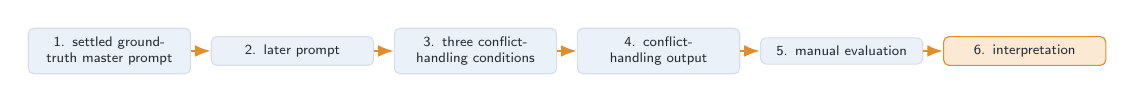
\begin{tikzpicture}[node distance=2.5mm]
    \node[flownode,inner sep=3pt,font=\tiny,text width=1.85cm,align=center] (q1) {1. settled ground-truth master prompt};
    \node[flownode,inner sep=3pt,font=\tiny,right=of q1,text width=1.85cm,align=center] (q2) {2. later prompt};
    \node[flownode,inner sep=3pt,font=\tiny,right=of q2,text width=1.85cm,align=center] (q3) {3. three conflict-handling conditions};
    \node[flownode,inner sep=3pt,font=\tiny,right=of q3,text width=1.85cm,align=center] (q4) {4. conflict-handling output};
    \node[flownode,inner sep=3pt,font=\tiny,right=of q4,text width=1.85cm,align=center] (q5) {5. manual evaluation};
    \node[flownode,inner sep=3pt,font=\tiny,right=of q5,fill=tintorange,draw=accentorange,text width=1.85cm,align=center] (q6) {6. interpretation};
    \draw[flowarrow] (q1)--(q2); \draw[flowarrow] (q2)--(q3); \draw[flowarrow] (q3)--(q4);
    \draw[flowarrow] (q4)--(q5); \draw[flowarrow] (q5)--(q6);
  \end{tikzpicture}
  \end{center}
  \vspace{10pt}
  \takeaway{5 semantic conflicts + 2 compatible controls.}
\end{frame}

\begin{frame}{What Counts as a Semantic Conflict?}
  \framesubtitle{Experiment 2 --- hard project}
  {\footnotesize\color{midgray}\textbf{Settled master prompt:} ``Invoice should have a due date \textbf{15 days} after they are created\dots''\par}
  \vspace{2pt}
  \begin{columns}[T]
    \begin{column}{0.49\textwidth}
      \begin{goodpanel}
        \textbf{\color{primaryblue}Clear Revision}\\[1pt]
        \calllbl{Example} ``Change the due date to 30 days.''\\[1pt]
        \calllbl{Meaning} The user replaces the settled 15-day value.\\[1pt]
        \calllbl{Action} Update the requirement.
      \end{goodpanel}
    \end{column}
    \begin{column}{0.49\textwidth}
      \begin{flagpanel}
        \textbf{\color{accentorange}Semantic Conflict}\\[1pt]
        \calllbl{Example} ``Add a reminder before the 30-day due date.''\\[1pt]
        \calllbl{Meaning} Assumes 30 days instead of settled 15-day value.\\[1pt]
        \calllbl{Action} Keep the settled requirement and report the conflict for users.
      \end{flagpanel}
    \end{column}
  \end{columns}
  \vspace{3pt}
  {\footnotesize\bfseries\color{accentorange}\centering Semantic conflict = an incompatible later assumption without a clear revision request.\par}
\end{frame}

\begin{frame}{Experiment 2: Controlled Prompts Setup}
  \framesubtitle{Experiment 2 --- Semantic Conflict Handling}
  {\small\bfseries\color{primaryblue}Starting point}
  \begin{center}
  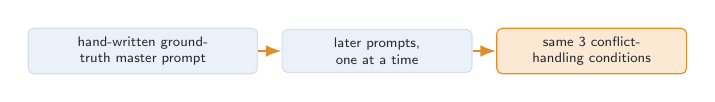
\begin{tikzpicture}[node distance=3mm]
    \node[flownode,inner sep=3pt,font=\tiny,text width=2.7cm,align=center] (h1) {hand-written ground-truth master prompt};
    \node[flownode,inner sep=3pt,font=\tiny,right=of h1,text width=2.2cm,align=center] (h2) {later prompts, one at a time};
    \node[flownode,inner sep=3pt,font=\tiny,right=of h2,fill=tintorange,draw=accentorange,text width=2.2cm,align=center] (h3) {same 3 conflict-handling conditions};
    \draw[flowarrow] (h1)--(h2); \draw[flowarrow] (h2)--(h3);
  \end{tikzpicture}
  \end{center}
  \vspace{2pt}
  \begin{columns}[T]
    \begin{column}{0.62\textwidth}
      {\scriptsize\bfseries\color{primaryblue}Hard project --- 4 semantic conflicts}
      \begin{itemize}\scriptsize
        \item \textbf{Due-date value} --- 15-day due date vs.\ assumed 30-day due date
        \item \textbf{Recycle-bin scope} --- vendors-only recycle bin vs.\ customer recycle-bin tab
        \item \textbf{Navigation layout} --- top navigation bar vs.\ collapsible left sidebar
        \item \textbf{Permission} --- staff cannot delete products vs.\ audit entry for staff deletions
      \end{itemize}
    \end{column}
    \begin{column}{0.36\textwidth}
      {\scriptsize\bfseries\color{primaryblue}Simple project --- 1 semantic conflict}
      \begin{itemize}\scriptsize
        \item \textbf{Navigation count} --- four navigation buttons vs.\ five buttons wrapping onto two rows
      \end{itemize}
      \vspace{2pt}
      {\scriptsize\bfseries\color{primaryblue}Compatible controls}
      \begin{itemize}\scriptsize
        \item Hard: print button
        \item Simple: footer note
      \end{itemize}
    \end{column}
  \end{columns}
  \vspace{1pt}
  {\scriptsize\bfseries\color{accentorange}\centering All agents and conditions receive the same settled specification and the same later prompts within each project.\par}
\end{frame}

\begin{frame}{Experiment 2: Conditions and Evaluation}
  \framesubtitle{Experiment 2 --- Semantic Conflict Handling}
  \begin{columns}[T]
    \begin{column}{0.5\textwidth}
      {\small\bfseries\color{primaryblue}Three Conditions}
      \begin{itemize}\scriptsize
        \item \textbf{Consolidate-then-ask} --- consolidate first, then inspect conflicts afterward.
        \item \textbf{Do-not-resolve} --- do not choose or merge conflicting values; keep the conflict separate.
        \item \textbf{Spec-guided} --- check each later prompt against the settled specification as it arrives.
      \end{itemize}
    \end{column}
    \begin{column}{0.48\textwidth}
      {\small\bfseries\color{primaryblue}Manual Evaluation}
      \begin{itemize}\scriptsize
        \item Detect the conflict
        \item Do not resolve it automatically
        \item Keep the settled requirement
        \item Do not invent new details
        \item Show both sources
      \end{itemize}
    \end{column}
  \end{columns}
  \vspace{6pt}
  \takeaway{Compatible additions should be accepted normally.}
\end{frame}

\begin{frame}{Gemini Output: Consolidate-Then-Ask}
  \framesubtitle{Experiment 2 --- simple project, Gemini \textperiodcentered\ navigation-count conflict}
  \begin{quotebox}
    \tiny
    \textbf{\color{primaryblue}Settled:} ``The navigation must contain four buttons: Dashboard, Policies, History, and Contact.''\\
    \textbf{\color{primaryblue}Later:} ``Make sure all five navigation buttons wrap onto two rows on small screens.''\\
    \textbf{\color{primaryblue}Later:} ``Add a footer at the bottom of the page showing a copyright notice.''\\[2pt]
    \textbf{\color{primaryblue}Output:} \textbf{Master prompt} --- ``Create a portal homepage. Add top navigation. The navigation must contain \textbf{five navigation buttons}, including Dashboard, Policies, History, and Contact. If the label of a navigation button starts with `H', its background color should be blue; if the label starts with `O', its background color should be red; if the label starts with `D', its background color should be yellow. Style the navigation with rounded buttons, a blue accent, and a modern font. Make sure all \textbf{five navigation buttons wrap onto two rows} on small screens. Add a contact form with name, email, and message fields. The email field must be validated before the form can submit. Make sure the page also works well on mobile screens. Add a footer at the bottom of the page showing a copyright notice.''\\[2pt]
    \textbf{Unresolved conflict}
    \vspace{-3pt}
    \begin{itemize}\tiny
      \item \textbf{Settled / Initial Requirement (Prompt 1):} ``The navigation must contain four buttons: Dashboard, Policies, History, and Contact.''
      \item \textbf{Later Instruction (Prompt 2):} ``Make sure all five navigation buttons wrap onto two rows on small screens.''
      \item \textbf{Conflict Analysis:} a navigation bar cannot contain both four and five buttons at once --- the later instruction raises the count from four to five.
    \end{itemize}
  \end{quotebox}
\end{frame}

\begin{frame}{Gemini Output: Do-Not-Resolve}
  \framesubtitle{Experiment 2 --- simple project, Gemini \textperiodcentered\ navigation-count conflict}
  \begin{quotebox}
    \scriptsize
    \textbf{\color{primaryblue}Settled:} ``The navigation must contain four buttons: Dashboard, Policies, History, and Contact.''\\[1pt]
    \textbf{\color{primaryblue}Later:} ``Make sure all five navigation buttons wrap onto two rows on small screens.''\\[1pt]
    \textbf{\color{primaryblue}Later:} ``Add a footer at the bottom of the page showing a copyright notice.''\\[2pt]
    \textbf{\color{primaryblue}Output:} \textbf{Master prompt} --- ``Create a portal homepage. Add top navigation. If the label of a navigation button starts with `H', its background color should be blue; if the label starts with `O', its background color should be red; if the label starts with `D', its background color should be yellow. Style the navigation with rounded buttons, a blue accent, and a modern font. Make sure navigation buttons wrap onto two rows on small screens. Add a contact form with name, email, and message fields. The email field must be validated before the form can submit. Make sure the page also works well on mobile screens. Add a footer at the bottom of the page showing a copyright notice.''\\[2pt]
    \textbf{Unresolved conflict} --- Number of Navigation Buttons \& Button List
    \vspace{-3pt}
    \begin{itemize}\scriptsize
      \item \textbf{Prompt 1:} ``The navigation must contain four buttons: Dashboard, Policies, History, and Contact.''
      \item \textbf{Prompt 2:} ``Make sure all five navigation buttons wrap onto two rows on small screens.''
    \end{itemize}
  \end{quotebox}
\end{frame}

\begin{frame}{Gemini Output: Spec-Guided Conflict Handling}
  \framesubtitle{Experiment 2 --- simple project, Gemini \textperiodcentered\ navigation-count conflict}
  \begin{quotebox}
    \scriptsize
    \textbf{\color{primaryblue}Settled:} ``The navigation must contain four buttons: Dashboard, Policies, History, and Contact.''\\[1pt]
    \textbf{\color{primaryblue}Later:} ``Make sure all five navigation buttons wrap onto two rows on small screens.''\\[1pt]
    \textbf{\color{primaryblue}Later:} ``Add a footer at the bottom of the page showing a copyright notice.''\\[2pt]
    \textbf{\color{primaryblue}Output:} \textbf{Master prompt} --- Create a portal homepage with top navigation, a contact form, and a footer.
    \vspace{-3pt}
    \begin{itemize}\tiny
      \item \textbf{Navigation Styling \& Behavior:} rounded buttons, blue accent, modern font; H$\to$blue, O$\to$red, D$\to$yellow; buttons wrap onto two rows on small screens.
      \item \textbf{Contact Form:} name, email, and message fields; email validated before the form can submit.
      \item \textbf{Footer:} copyright notice at the bottom of the page.
      \item \textbf{Responsiveness:} page works well on mobile screens.
    \end{itemize}
    \textbf{Unresolved conflict} --- Number of Navigation Buttons
    \vspace{-3pt}
    \begin{itemize}\tiny
      \item \textbf{Settled requirement:} ``The navigation must contain four buttons: Dashboard, Policies, History, and Contact.''
      \item \textbf{New prompt instruction:} ``Make sure all five navigation buttons wrap onto two rows on small screens.''
      \item \textbf{Why:} the initial prompt explicitly specifies four buttons, while a subsequent prompt specifies wrapping ``all five navigation buttons'' onto two rows without explicitly revising the button count or naming a fifth button.
    \end{itemize}
  \end{quotebox}
\end{frame}

\begin{frame}{Experiment 2: Interpretation and Key Challenge}
  \framesubtitle{Experiment 2 --- Semantic Conflict Handling}
  {\footnotesize\bfseries\color{primaryblue}Interpretation}
  \begin{itemize}\scriptsize
    \item \textbf{Consolidate-then-ask} --- the conflicting assumption can enter the Master Prompt before it is checked.
    \item \textbf{Do-not-resolve} --- keeps the conflicting value outside the Master Prompt.
    \item \textbf{Spec-guided} --- checks the later instruction before updating the settled specification, preserves the settled value, and asks the user.
  \end{itemize}
  \vspace{3pt}
  \begin{calloutbox}
    \footnotesize
    \calllbl{Key challenge --- revision or conflict?} A later prompt may introduce a new value without making it clear whether the user intended to revise the settled requirement.\\[3pt]
    \calllbl{Design response} If the revision is unclear, preserve the settled requirement and ask the user.
  \end{calloutbox}
  \vspace{4pt}
  {\small\bfseries\color{accentorange}\centering The main difference is when the conflict is checked: spec-guided checks the new instruction against the settled Master Prompt before changing it.\par}
\end{frame}

% ============================================================ SECTION 9 ==
\section{Conclusion}

\begin{frame}{Conclusion: Answers to the Research Questions}
  \framesubtitle{Conclusion}
  \small
  \begin{itemize}
    \item \textbf{RQ1} --- Explicit traceability constraints reduce non-traceable content in single-pass consolidation.
    \item \textbf{RQ2} --- Spec-guided improves 4/6 comparisons, but replaces one large reconstruction with repeated interpretation decisions.
    \item \textbf{RQ3} --- The qualitative conflict study shows that a settled specification can be used to surface incompatible later assumptions without silently resolving them.
  \end{itemize}
  \begin{calloutbox}
    \calllbl{Takeaway}A master prompt should be treated as a maintained project specification, not merely as a one-shot summary of prompt history.
  \end{calloutbox}
\end{frame}

\begin{frame}[plain,noframenumbering]
  \begin{center}
    \vfill
    {\color{primaryblue}\bfseries\huge Thank you}\\[10pt]
    {\color{accentorange}\rule{0.28\paperwidth}{1.4pt}}\\[10pt]
    {\color{midgray}\normalsize Time For Questions}
    \vfill
  \end{center}
\end{frame}

\end{document}
